\pdfminorversion=6
\pdfcompresslevel=9
\pdfobjcompresslevel=2

\documentclass[english,pdftex,dvipsnames,leqno,handout]{beamer}% handout option disables overlays
\mode<presentation>{\usetheme{CS-Saar-Uni}}

\usepackage[utf8]{inputenc}
\usepackage{babel}
\usepackage[T1]{fontenc}
\usepackage{lmodern} % HACK! This is a workaround for a bug in beamer that triggers in texlive 2017 with \tiny font, which in beamer goes to the untested/unsupported <5pt font (font generation of ecss0400 fails)


% Times/Helvetica/Courier combination
%\usepackage{mathptmx}
%\usepackage[scaled=.90]{helvet}
%\usepackage{courier}

% Palatino/Helvetica/Courier combination
%\usepackage{mathpazo}
%\usepackage[scaled=.95]{helvet}
%\usepackage{courier}

% Formatting
\usepackage{tabto} % provides \tab command

% Disable footnote ruler
\renewcommand{\footnoterule}{}

% Drawing
\usepackage{tikz}
% \usetikzlibrary{positioning,calc,decorations.pathreplacing}
% \usepackage{calc}
% \def\checkmark{\tikz\fill[scale=0.4](0,.35) -- (.25,0) -- (1,.7) -- (.25,.15) -- cycle;}
% \def\scalecheck{\resizebox{\widthof{\checkmark}*\ratio{\widthof{x}}{\widthof{\normalsize x}}}{!}{\checkmark}}

% \tikzstyle{every picture}+=[remember picture]
% \tikzstyle{na} = [baseline=-.5ex]

% \newcommand{\tikzmark}[1]{\tikz[overlay,remember picture] \node (#1) {};}

%colors from theme
\definecolor{sbdcyan}{RGB}{026, 058, 107}
\definecolor{sbmcyan}{RGB}{038, 116, 176}
\definecolor{sblcyan}{RGB}{109, 182, 218}
\definecolor{greenblue}{RGB}{0, 127, 79}

% Packages specific to the content
\usepackage{mathpartir}
\usepackage{xspace}
% \usepackage{mathpartir}
% \usepackage{ntheorem}

%%% MY MACROS, copy old if needed

% Formatting
\newcommand{\hl}[1]{\emph{\color{sbmcyan} #1}}
\newcommand{\mycite}[1]{{\color{greenblue}\scriptsize[#1]}}

% basic math
\newcommand{\NN}{\ensuremath{\mathbb{N}}}

% spacing
\newcommand{\ms}{\;\,}
\newcommand{\mbin}[1]{\mathbin{\ms #1 \ms}}
\newcommand{\mrel}[1]{\mathrel{\ms #1 \ms}} % meta level binary relation

% meta operators
\newcommand{\mForall}[1]{\forall #1.\ms}
\newcommand{\mExists}[1]{\exists #1.\ms}
\newcommand{\mIff}{\mrel{\iff}}
\newcommand{\mImpl}{\mrel{\Rightarrow}}
\newcommand{\mOf}{\mrel{:}}
\newcommand{\mAnd}{\mrel{\wedge}}
\newcommand{\mOr}{\mrel{\vee}}

% definitions
\newcommand{\eqdef}{\mbin{:=}}
\newcommand{\bnfdef}{\mbin{::=}}

% substitutions
\newcommand{\subst}[1]{\hphantom{|}\![{#1}]}
\newcommand{\id}{\mathsf{id}}
\newcommand{\shift}{\ensuremath{\uparrow}}
\newcommand{\up}{{\Uparrow}}
\newcommand{\scons}{\mathbin{\cdot}}
\newcommand{\scomp}{\mathbin{\circ}}

% adjusting relations
\newcommand{\cons}{\mathbin{\,:\hspace{-0.1em}:\,}}
\newcommand{\rup}[1]{\ensuremath{{#1}^\Uparrow}}
\newcommand{\rext}[1]{\ensuremath{{#1}^{\mathsf{ext}}}}

% systems
\newcommand{\SysF}{\ensuremath{\mathsf{\color{greenblue}F}}\xspace}
\newcommand{\SysL}{\ensuremath{{\color{sbmcyan}\lambda2}}\xspace}

\newcommand{\ty}{\mathsf{ty}}
\newcommand{\tm}{\mathsf{tm}}

% syntax
\newcommand{\TyF}{\ensuremath{\mathsf{\color{greenblue}Ty_{F}}}}
\newcommand{\TmF}{\ensuremath{\mathsf{\color{greenblue}Tm_{F}}}}

\newcommand{\impf}[2]{\ensuremath{#1 \mathbin{\color{greenblue}\rightarrow} #2}}
\newcommand{\allf}[1]{\ensuremath{{\color{greenblue}\forall.} #1}}
\newcommand{\nallf}[2]{\ensuremath{{\color{greenblue}\forall} #1 {\color{greenblue}.} #2}}
\newcommand{\appf}[2]{\ensuremath{#1 \mathop{\color{greenblue}\$} #2}}
\newcommand{\lamf}[2]{\ensuremath{{\color{greenblue}\lambda} #1 {\color{greenblue}.} #2}}
\newcommand{\tyappf}[2]{\ensuremath{#1 \mathop{\color{greenblue}@} #2}}
\newcommand{\tylamf}[1]{\ensuremath{{\color{greenblue}\Lambda.}#1}}
\newcommand{\ntylamf}[2]{\ensuremath{{\color{greenblue}\Lambda} #1 {\color{greenblue}.} #2}}

\newcommand{\TmL}{\ensuremath{\mathsf{\color{sbmcyan}Tm_{\lambda}}}}

\newcommand{\typl}{\ensuremath{{\color{sbmcyan}\square}}}
\newcommand{\prpl}{\ensuremath{\textrm{\color{sbmcyan}\textasteriskcentered}}}
\newcommand{\appl}[2]{\ensuremath{#1 \mathop{\color{sbmcyan}\$} #2}}
\newcommand{\laml}[2]{\ensuremath{{\color{sbmcyan}\lambda} #1 {\color{sbmcyan}.} #2}}
\newcommand{\prodl}[2]{\ensuremath{{\color{sbmcyan}\Pi} #1 {\color{sbmcyan}.} #2}}

% judgements
\newcommand{\of}{\mathbin{:}}
\newcommand{\tsf}{\mathrel{\color{greenblue}\vdash}}
\newcommand{\tsl}{\mathrel{\color{sbmcyan}\vdash}}

\newcommand{\istyf}[1]{\ensuremath{#1 \ms \mathbf{\color{greenblue}ty}}}
\newcommand{\typingf}[2]{\ensuremath{#1 \mathrel{\color{greenblue}\of_{\mathsf{F}}} #2}}

\newcommand{\univl}[1]{\ensuremath{\mathcal{\color{sbmcyan}U}\, #1}}
\newcommand{\typingl}[2]{\ensuremath{#1 \mathrel{\color{sbmcyan}\of_{2}} #2}}

\newcommand{\tyrel}[2]{\ensuremath{#1 \mathrel{\sim} #2}}
\newcommand{\tmrel}[2]{\ensuremath{#1 \mathrel{\approx} #2}}

% relational context morphisms
\newcommand{\tyctxrelFL}[3]{\ensuremath{#1\mathrel{\mathop{\longrightarrow}^{#2}\limits}#3}}
\newcommand{\tyctxrelLF}[3]{\ensuremath{#1\mathrel{\mathop{\longleftarrow}^{#2}\limits}#3}}
\newcommand{\tmctxrelFL}[4]{\ensuremath{#1\mathrel{\mathop{\longrightarrow}^{#2}_{#3}\limits}#4}}
\newcommand{\tmctxrelLF}[4]{\ensuremath{#1\mathrel{\mathop{\longleftarrow}^{#2}_{#3}\limits}#4}}

% LambdaProlog symbols
\newcommand{\lpProp}{\ensuremath{\mathbf{o}}}
\newcommand{\lpPi}[1]{\boldsymbol{\Pi} #1.\ms}
\newcommand{\lpApp}[2]{#1\langle#2\rangle}
\newcommand{\lpImp}{\mrel{=\!\blacktriangleright}}

% G Symbols
\newcommand{\gProp}{\ensuremath{\mathbf{Prop}}}


%%% END MACROS

% Generate Section Title Pages
% \AtBeginSection{\frame[noframenumbering]{\sectionpage}}
% \setbeamertemplate{section page}
% {
%   \begin{centering}
%     \begin{beamercolorbox}[sep=4pt,center]{part title}
%       \usebeamerfont{section title}\insertsection\par
%     \end{beamercolorbox}
%   \end{centering}
% }

%%%%%%%%%%%%%%%%%%%%%%%%%%%%%%%%%%%%%%%%%%%%%%%%%%%%%%%%%%%%%%%%%%%%%%%%%%%%%%%%
% Metadata
%%%%%%%%%%%%%%%%%%%%%%%%%%%%%%%%%%%%%%%%%%%%%%%%%%%%%%%%%%%%%%%%%%%%%%%%%%%%%%%%
\title[$F$ and $\lambda 2$ -- A Case Study]{Relating System F and $\lambda2$:\\A Case Study in Coq, Abella and Beluga}
%\subtitle{}

\author[Jonas Kaiser]{
  \texorpdfstring{
    \href{http://www.ps.uni-saarland.de/~jkaiser}{\underline{Jonas Kaiser}} \and
    \href{http://www.cs.mcgill.ca/~bpientka}{Brigitte Pientka} \and
    \href{http://www.ps.uni-saarland.de/~smolka}{Gert Smolka}
  }
  {Jonas Kaiser}}

\institute[Saarland University]{\normalsize FSCD 2017, Oxford}

\date{September 4, 2017}

%%%%%%%%%%%%%%%%%%%%%%%%%%%%%%%%%%%%%%%%%%%%%%%%%%%%%%%%%%%%%%%%%%%%%%%%%%%%%%%%
% Content
%%%%%%%%%%%%%%%%%%%%%%%%%%%%%%%%%%%%%%%%%%%%%%%%%%%%%%%%%%%%%%%%%%%%%%%%%%%%%%%%

\begin{document}

\section*{Introduction}

\begin{frame}[plain]
  \titlepage
\end{frame}

\begin{frame}
  \frametitle{Overview}
  \tableofcontents
\end{frame}

\section{Variants of System F}

\begin{frame}
  \frametitle{System F \mycite{Girard '72} / PTLC \mycite{Reynolds '74}}
  \structure{Some History}
  \begin{itemize}
  \item Developed in the context of proof theory and polymorphism.
  \item Commonly phrased as a {\color{greenblue}two-sorted} system:
    \begin{itemize}
    \item Types
    \item Terms
    \end{itemize}
  \item We consider \SysF as presented in \mycite{Harper '13}.
    \begin{itemize}
    \item Explicitly scopes type variables.
    \end{itemize}
  \end{itemize}
  \structure{Meanwhile\ldots}
  \begin{itemize}
  \item Study of CC led to {\color{sbmcyan}single-sorted} Pure Type Systems (PTS):
    \begin{itemize}
    \item The $\lambda$-cube of \mycite{Barendregt '91}.
    \end{itemize}
  \item System~F appears as the corner $\SysL$.
  \end{itemize}
  \structure{The Question}
  \begin{center}
    $\SysF \quad \leftrightsquigarrow \quad\SysL$\\
    \emph{bidirectional reduction of typing}
  \end{center}
\end{frame}

% \begin{frame}
%   \frametitle{Introduction}
%   \begin{block}{1) The Mathematical Problem}
%     \begin{itemize}
%     \item Several variants of System F \mycite{Girard '72} / PTLC \mycite{Reynolds '74} exist.
%     \item In particular
%       \begin{itemize}
%       \item $\SysF$ -- two-sorted with explicit type variable context \mycite{Harper '13}
%       \item $\SysL$ -- single-sorted pure type system (PTS) style \mycite{Barendregt '91}
%       \end{itemize}
%     \item Transport of results relies on correspondence, e.g.\ \hl{reduction of typing}.
%     \end{itemize}
%   \end{block}
%   \pause
%   \begin{block}{2) The Formalisation Problem}
%     \begin{itemize}
%     \item Syntax with binders.
%     \item Representation of variables.
%     \item Tracking of contextual information.
%     \end{itemize}
%   \end{block}
% \end{frame}

\begin{frame}
  \frametitle{Syntactic Variants $\SysF$ and $\SysL$}
  Two-sorted non-uniform syntax:
  \begin{align*}
    &\TyF & A, B \bnfdef &X \mid \impf{A}{B} \mid \nallf{X}{A} \\
    &\TmF & s, t \bnfdef &x \mid \appf{s}{t} \mid \lamf{x \of A}{s} \mid \tyappf{s}{A} \mid \ntylamf{X}{s}\\[.6em]
    &\textup{\color{greenblue}Type  Formation} & &\Delta \tsf \istyf{A} \\
    &\textup{\color{greenblue}Typing} & &\Delta; \Gamma \tsf \typingf{s}{A} \\
    \intertext{Single-sorted uniform PTS syntax:}
    &\TmL & a, b \bnfdef &x \mid \prpl \mid \typl \mid \appl{a}{b} \mid \laml{x \of a}{b} \mid \prodl{x \of a}{b}\\[.6em]
    &\textup{\color{sbmcyan}Typing} & & \Psi \tsl \typingl{a}{b}
  \end{align*}
\end{frame}

\begin{frame}
  \frametitle{Syntactic Correspondence}
  \begin{center}
    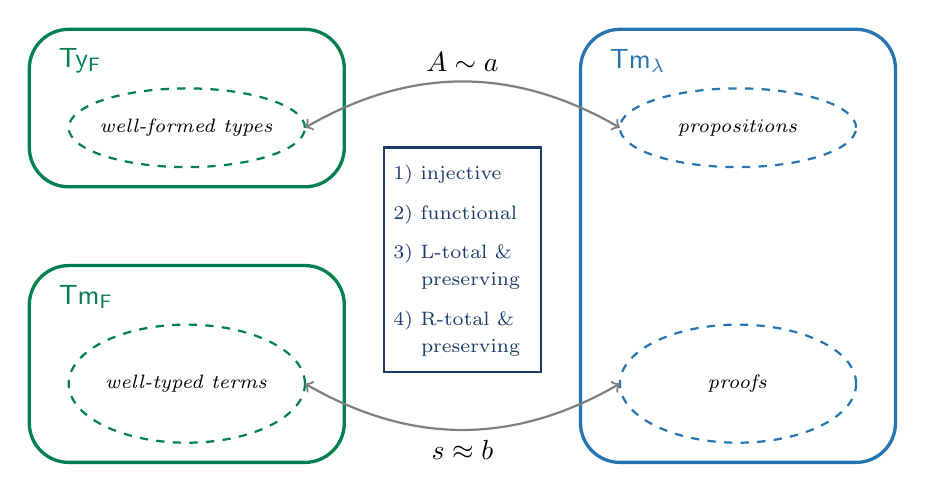
\begin{tikzpicture}
      %\draw[step=.5cm,gray,very thin] (0,0) grid (12,7);
      \draw[rounded corners=.5cm,very thick,greenblue] (.5,4.5) rectangle (4.5,6.5);
      \node[right] at (.75,6.1) {$\TyF$};
      \draw[dashed,greenblue,thick] (2.5,5.25) ellipse (1.5cm and .5cm);
      \node at (2.5,5.25) {\textit{\scriptsize well-formed types}};
      \draw[rounded corners=.5cm,very thick,greenblue] (.5,1) rectangle (4.5,3.5);
      \node[right] at (.75,3.1) {$\TmF$};
      \draw[dashed,greenblue,thick] (2.5,2) ellipse (1.5cm and .75cm);
      \node at (2.5,2) {\textit{\scriptsize well-typed terms}};
      \draw[rounded corners=.5cm,very thick,sbmcyan] (7.5,1) rectangle (11.5,6.5);
      \node[right] at (7.75,6.1) {$\TmL$};
      \draw[dashed,sbmcyan,thick] (9.5,5.25) ellipse (1.5cm and .5cm);
      \node at (9.5,5.25) {\textit{\scriptsize propositions}};
      \draw[dashed,sbmcyan,thick] (9.5,2) ellipse (1.5cm and .75cm);
      \node at (9.5,2) {\textit{\scriptsize proofs}};
      \draw[<->,thick,gray] (4,5.25) to[bend left] node[above] {\color{black}$A \sim a$} (8,5.25);
      \draw[<->,thick,gray] (4,2) to[bend right] node[below] {\color{black}$s \approx b$} (8,2);
      \draw[sbdcyan,thick] (5,2.15) rectangle (7,5);
      \node[sbdcyan,right] at (5,4.65) {\scriptsize 1) injective};
      \node[sbdcyan,right] at (5,4.15) {\scriptsize 2) functional};
      \node[sbdcyan,right] at (5,3.65) {\scriptsize 3) L-total \&};
      \node[sbdcyan,right] at (5.35,3.3) {\scriptsize preserving};
      \node[sbdcyan,right] at (5,2.8) {\scriptsize 4) R-total \&};
      \node[sbdcyan,right] at (5.35,2.45) {\scriptsize preserving};
    \end{tikzpicture}
  \end{center}
\end{frame}

\begin{frame}
  \frametitle{Syntactic Correspondence, Complications}
  \begin{itemize}
  \item Non-uniform vs.\ uniform:
    \vspace{1em}
    \begin{center}
      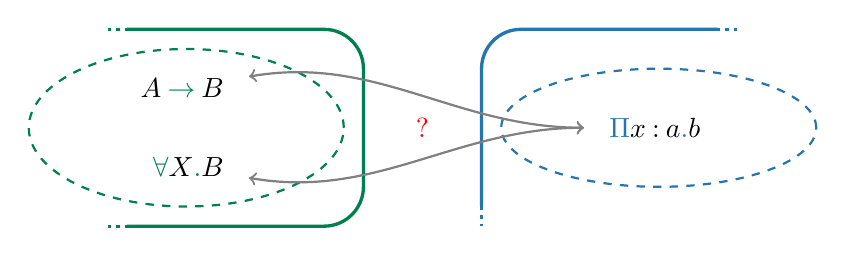
\begin{tikzpicture}
        %\draw[step=.5cm,gray,very thin] (0,0) grid (11,3);
        \draw[dotted,very thick,greenblue] (1.5,2.75) -- (1.75,2.75);
        \draw[rounded corners=.5cm,very thick,greenblue] (1.75,2.75) -- (4.75,2.75) -- (4.75,0.25) -- (1.75,0.25);
        \draw[dotted,very thick,greenblue] (1.5,0.25) -- (1.75,0.25);
        \draw[dashed,greenblue,thick] (2.5,1.5) ellipse (2cm and 1cm);
        \node[left] (L1) at (3.1,2) {$\impf{A}{B}$};
        \node[left] (L2) at (3.1,1) {$\nallf{X}{B}$};
        \draw[dotted,very thick,sbmcyan] (9.5,2.75) -- (9.25,2.75);
        \draw[rounded corners=.5cm,very thick,sbmcyan] (9.25,2.75) -- (6.25,2.75) -- (6.25,0.5);
        \draw[dotted,very thick,sbmcyan] (6.25,0.5) -- (6.25,0.25);
        \draw[dashed,sbmcyan,thick] (8.5,1.5) ellipse (2cm and .75cm);
        \node[right] (R) at (7.75,1.5) {$\prodl{x \of a}{b}$};
        \draw[<->,thick,gray,shorten <= .2cm, shorten >= .2cm] (L1) to[out=10,in=180] (R);
        \draw[<->,thick,gray,shorten <= .2cm, shorten >= .2cm] (L2) to[out=-10,in=180] (R);
        \node[red] at (5.5,1.5) {?};
      \end{tikzpicture}
    \end{center}
    \vspace{1em}
  \item Open terms \& contextual assumptions about
    \begin{itemize}
    \item \hl{well-formedness}: \tabto{0.3\linewidth} in $\impf{X}{X}$, is $X$ in scope?
    \item \hl{typing}: \tabto{0.3\linewidth} in $\appl{a}{b}$, is $b$ a proof or proposition?
    \item \hl{related variables}: \tabto{0.3\linewidth} in the var case, does  $\Theta \vdash X \sim x$ hold?
    \end{itemize}
  \item Aligning the binding structures.
    \begin{itemize}
    \item Some \SysL products are vacuous.
    \item Two variable scopes for \SysF vs.\ unified scope for \SysL.
    \end{itemize}

  \end{itemize}
\end{frame}

\begin{frame}
  \frametitle{The Reduction Proof ($\SysF \leftrightsquigarrow \SysL$)}
  Assume we are given syntactic relations $\sim$ and $\approx$ which are both:
  \begin{enumerate}
  \item functional
  \item injective
  \item left-total and judgement preserving on suitable fragment
  \item right-total and judgement preserving on suitable fragment
  \end{enumerate}
  \begin{theorem}[Reduction $\SysF \rightsquigarrow \SysL$]\vspace{-2em}
    \begin{align*}
      {} \tsf \istyf{A} &\mIff \mExists a \tyrel{A}{a} \mAnd {} \tsl \typingl{a}{\prpl}\\
      {} \tsf \typingf{s}{A} &\mIff \mExists{b,a} \tmrel{s}{b} \mAnd \tyrel{A}{a} \mAnd {} \tsl \typingl{b}{a} \mAnd {} \tsl \typingl{a}{\prpl}
    \end{align*}
    \vspace{-1.8em}
  \end{theorem}
  \begin{theorem}[Reduction $\SysL \rightsquigarrow \SysF$]\vspace{-1.8em}
    \begin{align*}
      {} \tsl \typingl{a}{\prpl} &\mIff \mExists A \tyrel{A}{a} \mAnd {} \tsf \istyf{A}\\
      {} \tsl \typingl{b}{a} \mAnd {} \tsl \typingl{a}{\prpl} &\mIff \mExists {s,A} \tmrel{s}{b} \mAnd \tyrel{A}{a} \mAnd {} \tsf \typingf{s}{A}
    \end{align*}
    \vspace{-1.8em}
  \end{theorem}
\end{frame}


\begin{frame}
  \frametitle{Related Work}
  \pause
  \begin{itemize}
  \item The reduction result is partially discussed in \mycite{Geuvers '93}.
    \begin{itemize}
    \item Primarily argues the forward preservation of typing.
    \item The syntactic correspondence ($\sim$/$\approx$) is left implicit.
    \end{itemize}\pause
  \item We give a Coq formalisation of the full reduction in \mycite{K/Tebbi/Smolka '17}.
    \begin{itemize}
    \item Pairs of translation functions establish the syntactic correspondence.
    \item Requires involved cancellation laws.
    \item Proofs based on an extension of context morphism lemmas \mycite{Goguen/McKinna '97, Adams '06}.
    \end{itemize}
  \end{itemize}
\end{frame}

\section{The Equivalence Proof}

\begin{frame}
  \frametitle{Overview of the Proof}
  \begin{itemize}
  \item \hl{Step 1:} Define $\sim$ and $\approx$ as inductive relations.\pause
  \item \hl{Step 2:} Establish the following \hl{six properties} of $\sim$ and $\approx$:
    \begin{enumerate}
    \item $\sim$ is functional and injective.
    \item $\sim$ is L-total and type-formation preserving on well-formed types of $\SysF$.
    \item $\sim$ is R-total and type-formation preserving on propositions of $\SysL$.
    \item $\approx$ is functional and injective.
    \item $\approx$ is L-total and typing preserving on well-typed terms of $\SysF$.
    \item $\approx$ is R-total and typing preserving on proofs of $\SysL$.
    \end{enumerate}\pause
  \item \hl{Step 3:} Derive from these the four equivalences that together establish the reduction result.
  \end{itemize}\pause
  \begin{center}
    \hl{Observation:}\\
    L/R-totality are only required for a sensible fragment of the respective language.
    On these fragments we effectively\\ obtain a 1--1 correspondence.
  \end{center}
\end{frame}

\begin{frame}
  \frametitle{Relating the Types, $\tyrel{A}{a}$}
  \begin{mathpar}
    \inferrule*{(X,y) \in \Theta}{\Theta \vdash \tyrel{X}{y}} \\
    \inferrule*[right=$y \notin \Theta$]{\Theta \vdash \tyrel{A}{a} \\ \Theta \vdash \tyrel{B}{b}}{\Theta \vdash \tyrel{\impf{A}{B}}{\prodl{y \of a}{b}}} \\
    \inferrule*[right={$X,y \notin \Theta$}]{\Theta, (X,y) \vdash \tyrel{A}{a}}{\Theta \vdash \tyrel{\nallf{X}{A}}{\prodl{y \of \prpl}{a}}}
  \end{mathpar}
\end{frame}

\begin{frame}
  \frametitle{Relating the Terms, $\tmrel{s}{b}$}
  \begin{mathpar}
    \inferrule*{(x,y) \in \Sigma}{\Theta;\Sigma \vdash \tmrel{x}{y}} \\
    \inferrule*{\Theta;\Sigma \vdash \tmrel{s}{a} \\ \Theta;\Sigma \vdash \tmrel{t}{b}}{\Theta;\Sigma \vdash \tmrel{\appf{s}{t}}{\appl{a}{b}}} \and
    \inferrule*{\Theta;\Sigma \vdash \tmrel{s}{a} \\ \Theta \vdash \tyrel{A}{b}}{\Theta;\Sigma \vdash \tmrel{\tyappf{s}{A}}{\appl{a}{b}}} \\
    \inferrule*[right={$x,y \notin \Theta,\Sigma$}]{\Theta \vdash \tyrel{A}{a} \\ \Theta;\Sigma, (x,y) \vdash \tmrel{s}{b}}{\Theta;\Sigma \vdash \tmrel{\lamf{x \of A}{s}}{\laml{y \of a}{b}}} \\
    \inferrule*[right={$X,y \notin \Theta,\Sigma$}]{\Theta, (X,y);\Sigma \vdash \tmrel{s}{a}}{\Theta;\Sigma \vdash \tmrel{\ntylamf{X}{s}}{\laml{y \of \prpl}}{a}}
  \end{mathpar}
\end{frame}


\begin{frame}
  \frametitle{The Proof}
  \pause
  \begin{itemize}
  \item The six properties:
    \begin{itemize}
    \item Rely on some system-local meta-theoretic properties, e.g.:
      \begin{itemize}
      \item Propagation: $\Delta,\Gamma \tsf \typingf{s}{A} \mImpl \Delta \tsf \istyf{A}$.
      \item Degeneracy of $\typl$: $\Psi \tsl \typingl{a}{\typl} \mImpl a = \prpl$.
      \item \ldots
      \end{itemize}
    \item Interaction of various contexts: $\Delta, \Gamma, \Psi, \Theta, \Sigma$.
    \item The direction $\SysL \leadsto \SysF$ is harder, as structure has to be recovered.
    \end{itemize}\pause
  \item Deriving the equivalences, e.g.:
    \begin{align*}
      {} \tsf \istyf{A} &\mIff \mExists a \tyrel{A}{a} \mAnd {} \tsl \typingl{a}{\prpl}
    \end{align*}
    \vspace{-1.4em}\pause
    \begin{itemize}
    \item Proof ($\Rightarrow$): Immediate from L-totality and preservation of $\sim$.
    \item Proof ($\Leftarrow$): R-totality and preservation of $\sim$ on ${} \tsl \typingl{a}{\prpl}$ yields an $A'$ with $\tyrel{A'}{a}$ and ${} \tsf \istyf{A'}$.
      Injectivity of $\sim$ entails $A = A'$.
    \end{itemize}\pause
  \item The other three equivalences are similar.
  \end{itemize}
\end{frame}

\section{Formalisation}

\begin{frame}
  \frametitle{Formalising the Proof}
  \structure{How \ldots}\pause
  \begin{itemize}
  \item \ldots do we formally represent the syntax and judgements?\pause
  \item \ldots do we manage local variable binding?\pause
  \item \ldots track various pieces of contextual information?\pause
  \end{itemize}
  \structure{In various proof assistants:}\pause
  \begin{itemize}
  \item Coq
  \item Abella
  \item Beluga
  \end{itemize}
\end{frame}

\subsection{de Bruijn -- Coq}

\begin{frame}
  \begin{center}
    \begin{Large}
      \hl{-- Coq --\\[1em]An Index For An Index}
    \end{Large}\\[2em]
    de Bruijn, Parallel Substitutions, DIY Invariants
  \end{center}
\end{frame}

\begin{frame}
  \frametitle{Coq -- Representation}
  \begin{itemize}
  \item First order de Bruijn encoding, e.g.:
    \begin{align*}
      A, B \bnfdef &n_\ty \mid \impf{A}{B} \mid \allf{A} & &n \in \NN \\
      s, t \bnfdef &n_\tm \mid \appf{s}{t} \mid \lamf{A}{s} \mid \tyappf{s}{A} \mid \tylamf{s} & &
    \end{align*}\pause
  \item Typing contexts:
    \begin{align*}
      \Delta &\mOf \NN & &\textup{-- \hl{excl.\ upper bound for free type vars}}\\
      \Gamma &\mOf \mathsf{list}\;\TyF & &\textup{-- \hl{dangling term vars reference by position}}
    \end{align*}\pause
  \item Parallel substitutions $\sigma \of \NN \to \mathcal{T}$:
    \begin{align*}
      (\allf{A})\subst{\sigma} & \leadsto \allf{A\subst{\up\sigma}} & \up\sigma &\eqdef 0_\ty \scons \sigma \scomp \shift
    \end{align*}\pause
  \item Instantiation generated with \hl{Autosubst} library \mycite{Schäfer/Tebbi/Smolka '15}.
  \end{itemize}
\end{frame}

\begin{frame}
  \frametitle{Coq -- Relating Indices}
  \begin{itemize}
  \item Relating open terms requires tracking of related indices:
    \begin{align*}
      R, S \of \mathsf{list}\;(\NN \times \NN)
    \end{align*}\pause
  \item Traversal of binders requires context adjustments:
    \begin{mathpar}
      \inferrule*{R \vdash \tyrel{A}{a} \\ {\color{red}\rup{R}} \vdash \tyrel{B}{b}}{R \vdash \tyrel{\impf{A}{B}}{\prodl{a}{b}}} \and
      \inferrule*{{\color{red}\rext{R}} \vdash \tyrel{A}{a}}{R \vdash \tyrel{\allf{A}}{\prodl{\prpl}{a}}}
    \end{mathpar}\pause
    \begin{align*}
      {\color{red}\rext{R}} &\eqdef (0,0) \cons \mathsf{map}\,\,(\shift \times \shift)\,\,R\\
      {\color{red}\rup{R}} &\eqdef \mathsf{map}\,\,(\id\, \times \shift)\,\,R\\
    \end{align*}\pause
    \vspace{-2em}
    \begin{mathpar}
      \inferrule*{R \vdash \tyrel{A}{a} \\ {\color{red}\rup{R};\rext{S}} \vdash \tmrel{s}{b}}{R;S \vdash \tmrel{\lamf{A}{s}}{\laml{a}{b}}}
    \end{mathpar}
  \end{itemize}
\end{frame}

\begin{frame}
  \frametitle{Coq -- Context Managment, Proofs of P1 and P4.}
  \begin{itemize}
  \item $\rext{R}$ and $\rup{R}$ preserve injectivity and functionality of $R$.\pause
  \item Inj/func of $R$ entails  inj/func of $R \vdash \tyrel{\_}{\_}$. \hl{(P1)}\pause
  \item Func of $R, S$ entails func of $R;S \vdash \tmrel{\_}{\_}$. \hl{(P4a)}\pause
  \item Write $R \parallel S$ for $R$ and $S$ having disjoint ranges.
    \begin{itemize}
    \item W.l.o.g.: $R \parallel S \mImpl \rup{R} \parallel \rext{S}$.
    \item $R \parallel S \mImpl \neg (R \vdash \tyrel{A}{a} \mAnd R;S \vdash \tmrel{s}{a})$.
    \end{itemize}\pause
  \item Inj of $R,S$ and $R \parallel S$ entail inj of $R;S \vdash \tmrel{\_}{\_}$. \hl{(P4b)}
  \end{itemize}
\end{frame}

\begin{frame}
  \frametitle{Coq -- Proof of P2, custom invariants}
  \begin{itemize}
  \item P2: L-totality and preservation of type formation for $\sim$.\pause
  \item Recall the core idea of \hl{context morphism lemmas}:
    \begin{enumerate}
    \item Specify desired property on variables of initial context.
    \item Prove closure of property under context extensions.
    \item Lift property inductively to judgements.
    \end{enumerate}\pause
  \item Let $\tyctxrelFL{\Delta}{R}{\Psi} \eqdef \mForall{x < \Delta} \mExists y (x,y) \in R \mAnd (\typingl{y}{\prpl}) \mathrel{\in_\lambda} \Psi$.
    \begin{align*}
      \tyctxrelFL{\Delta}{R}{\Psi} &\mImpl \tyctxrelFL{\Delta}{\rup{R}}{\Psi,a} & &\textup{(ext.\ with new term var)}\\
      \tyctxrelFL{\Delta}{R}{\Psi} &\mImpl \tyctxrelFL{\Delta+1}{\rext{R}}{\Psi,\prpl} & &\textup{(ext.\ with new type var)}
    \end{align*}\pause
  \item Prove \hl{(P2)} by induction on $\Delta \tsf \istyf{A}$:
    \begin{align*}
      \Delta \tsf \istyf{A} \mImpl \mForall {R,\Psi} \tyctxrelFL{\Delta}{R}{\Psi} \mImpl \mExists a R \vdash \tyrel{A}{a} \mAnd \Psi \tsl \typingl{a}{\prpl}
    \end{align*}\pause
  \item Repeat similarly for \hl{(P3)}, \hl{(P5)} and \hl{(P6)}.
  \end{itemize}
\end{frame}

\subsection{HOAS/$\nabla$  -- Abella}

\begin{frame}
  \begin{center}
    \begin{Large}
      \hl{-- Abella --\\[1em]Inversions Galore!}
    \end{Large}\\[2em]
    HOAS, two-level logic, $\nabla$-quantification, relational proof search
  \end{center}
\end{frame}

\begin{frame}
  \frametitle{Abella \mycite{Miller, Chaudhuri et al.\ '14}}
  \begin{itemize}
  \item Two-level logic:\pause
    \begin{itemize}
    \item \hl{Specification Level:} $\lambda$Prolog, HOAS, logic predicates, proof search
      \begin{align*}
        &\lamf{\_}{\_} \mOf \TyF \to (\TmF \to \TmF) \to \TmF\\
        &\typingf{\_}{\_} \mOf \TmF \to \TyF \to \lpProp
      \end{align*}\pause
    \item \hl{Reasoing Level:} $\mathcal{G}$ -- intuitionistic, predicative, STT, $\nabla$-quantification
      \begin{align*}
        \nabla x.\ms \nabla y. \ms x \neq y
      \end{align*}
    \end{itemize}\pause
  \item Logical Embedding $\{\_ \vdash \_\} \mOf [\lpProp] \to \lpProp \to \gProp$\pause
    \begin{itemize}
    \item $\{L \vdash J\}$ holds in $\mathcal{G}$ iff $J$ has a $\lambda$Prolog-derivation, given hypotheses $L$.
    \item Exposes inductive structure of derivations.
    \end{itemize}
  \end{itemize}
\end{frame}

\begin{frame}
  \frametitle{Abella - Syntactic Relations as Logical Predicates}
  \begin{align*}
    \tyrel{\_}{\_} &\mOf \TyF \to \TmL \to \lpProp & \tmrel{\_}{\_} &\mOf \TmF \to \TmL \to \lpProp
  \end{align*}\pause
  \begin{mathpar}
    \inferrule*{\tyrel{A}{a} \\ \lpPi {x} \tyrel{B}{\lpApp{b}{x}}}{\tyrel{\impf{A}{B}}{\prodl{a}{b}}} \and
    \inferrule*{\lpPi {x\,y} \tyrel{x}{y} \lpImp \tyrel{\lpApp{A}{x}}{\lpApp{a}{y}}}{\tyrel{\allf{A}}{\prodl{\prpl}{a}}}
  \end{mathpar}\pause
  \begin{mathpar}
    \inferrule*{\tmrel{s}{a} \\ \tmrel{t}{b}}{\tmrel{\appf{s}{t}}{\appl{a}{b}}}\and
    \inferrule*{\tyrel{A}{a} \\ \lpPi {x\,y} \tmrel{x}{y} \lpImp \tmrel{\lpApp{s}{x}}{\lpApp{b}{y}}}{\tmrel{\lamf{A}{s}}{\laml{a}{b}}} \\
    \inferrule*{\tmrel{s}{a} \\ \tyrel{B}{b}}{\tmrel{\tyappf{s}{B}}{\appl{a}{b}}}\and
    \inferrule*{\lpPi {x\,y} \tyrel{x}{y} \lpImp \tmrel{\lpApp{s}{x}}{\lpApp{b}{y}}}{\tmrel{\tylamf{s}}{\laml{\prpl}{b}}}
  \end{mathpar}
\end{frame}

\begin{frame}
  \frametitle{Abella - Embedding, Instantiation \& Cut}
  \structure{Embedding example (recall premise of rule for \tmrel{\tylamf{s}}{\laml{\prpl}{b}}):}
  \begin{align*}
    &\{ L \vdash \lpPi {x\,y} \tyrel{x}{y} \lpImp \tmrel{\lpApp{s}{x}}{\lpApp{b}{y}}\} \\
    \leadsto \quad &\nabla x,y. \{ L \vdash \tyrel{x}{y} \lpImp \tmrel{\lpApp{s}{x}}{\lpApp{b}{y}}\}\\
    \leadsto \quad &\nabla x,y. \{ L, \tyrel{x}{y} \vdash \tmrel{\lpApp{s}{x}}{\lpApp{b}{y}}\} \\
    \leadsto \quad &\{ L, \tyrel{n_1}{n_2} \vdash \tmrel{\lpApp{s}{n_1}}{\lpApp{b}{n_2}}\}
  \end{align*}\pause
  \structure{Reasoning in $\mathcal{G}$ with Instantiation \& Cut:}\pause
  \begin{mathpar}
    \inferrule*[right=cut]{\{ L \vdash \tyrel{A}{a}\} \\ \inferrule*[right=inst]{\{ L, \tyrel{n_1}{n_2} \vdash  \tmrel{\lpApp{s}{n_1}}{\lpApp{b}{n_2}}\}}{\{ L, \tyrel{A}{a} \vdash \tmrel{\lpApp{s}{A}}{\lpApp{b}{a}}\}}}{\{ L \vdash \tmrel{\lpApp{s}{A}}{\lpApp{b}{a}}\}}
  \end{mathpar}
\end{frame}

\begin{frame}
  \frametitle{Abella -- Context Management}
  \begin{itemize}
  \item Contexts $L \of [\lpProp]$ are lists of arbitrary logical predicate instances.\pause
  \item The embedding has a backchaining rule \hl{$J \in L \mImpl \{L \vdash J\}$}.\pause
  \item We want typing/relational contexts that only contain information about variables, i.e.\ \hl{nominals}. \pause $\Rightarrow$ Inductive $\mathcal{G}$-predicates:
    {\color{greenblue}\begin{align*}
                        \mathsf{Define}\; &C_\approx \of [\lpProp] \to \gProp\;\mathsf{by}\\
                                          &C_\approx(\bullet);\\
                                          &\nabla x\,y,\ms C_\approx(L, \tyrel{x}{y}) \eqdef C_\approx(L);\\
                                          &\nabla x\,y,\ms C_\approx(L, \tmrel{x}{y}) \eqdef C_\approx(L).
    \end{align*}}\vspace{-1.6em}\pause
    \item Use {\color{greenblue}$C_\approx(L)$} to establish several inversion lemmas that discard spurious instances of backchaining. Required for \hl{(P1)} and \hl{(P4)}.\pause
    \item \hl{Note 1:} {\color{greenblue}$C_\approx(L)$} constrains $L$ to exactly track related variables. \pause
    \item \hl{Note 2:} {\color{greenblue}$C_\approx(L)$} forces $L$ to be injective, functional \& range-disjoint.
  \end{itemize}
\end{frame}

\begin{frame}
  \frametitle{Abella -- Proof of P2, More Inversions}
  \begin{itemize}
  \item L-totality \& preservation of type formation \hl{(P2)}:
    \begin{align*}
      \{L_F \vdash \istyf{A}\} \mImpl \mForall {L_\approx \, L_2} &C_R(L_F \mid L_\approx \mid L_2) \mImpl\\
      & \mExists {a} \{L_\approx \vdash \tyrel{A}{a}\} \mAnd \{L_2 \vdash \typingl{a}{\prpl}\}
    \end{align*}\pause
    \begin{mathpar}
      \inferrule*{~}{C_R(\bullet \mid \bullet \mid \bullet)} \and
      \inferrule*{C_R(L_F \mid L_\approx \mid L_2) \\ {\color{sblcyan}x,y\;\textup{fresh for}\;L_F,L_\approx,L_2}}{C_R(L_F, \istyf{x} \mid L_\approx, \tyrel{x}{y} \mid L_2,\typingl{y}{\prpl})} \\
      \inferrule*{\{L_F \vdash \istyf{A}\} \\ \{L_\approx \vdash \tyrel{A}{a} \}\\ \{L_2 \vdash \typingl{a}{\prpl}\} \\\\ C_R(L_F \mid L_\approx \mid L_2) \\ {\color{sblcyan}x,y\;\textup{fresh for}\;L_F,L_\approx,L_2,A,a}}{C_R(L_F, \typingf{x}{A} \mid L_\approx, \tmrel{x}{y} \mid L_2, \typingl{y}{a})}
    \end{mathpar}\pause
  \item $C_R(L_F \mid L_\approx \mid L_2)$ ensures that $L_\approx$ precisely relates $L_F$ and $L_2$, e.g.:
    \begin{align*}
      C_R(L_F \mid & L_\approx \mid L_2) \mImpl \tyrel{x}{y} \in L_\approx \mImpl \\
      &\istyf{x} \in L_F \mAnd \typingl{y}{\prpl} \in L_2 \mAnd \textup{"$x$ and $y$ are \hl{nominals}"}
    \end{align*}
  \end{itemize}
\end{frame}

\subsection{HOAS/CMTT -- Beluga}
% special remark:  context schemas not always inferrable, due to rather specific requirements (e.g. x : *), contrary to common believe.

\begin{frame}
  \begin{center}
    \begin{Large}
      \hl{-- Beluga --\\[1em]Give Me Some (Specific) Context, Please!}
    \end{Large}\\[2em]
    HOAS, contextual modal type theory, context schemas, proof terms
  \end{center}
\end{frame}

\begin{frame}
  \frametitle{Beluga -- Contextual Objects}
  \begin{itemize}
  \item Objects $K$ (types, terms, derivations) paired with a 1$^{st}$-class context $\Gamma$:
    \begin{align*}
      [\Gamma \vdash K]
    \end{align*}\pause
  \item No concept of \hl{free variable}: \pause
    \begin{itemize}
    \item In Coq: $0 \tsf \istyf{\impf{0_\ty}{0_\ty}} \mImpl \bot$ provable. \pause
    \item In Abella: $\{\bullet \vdash \istyf{\impf{n_0}{n_0}} \}\mImpl \bot$ provable. \pause
    \item In Beluga $[\bullet \vdash \istyf{\impf{x}{x}}]$ syntactically ill-formed since $x \notin \bullet$.
    \end{itemize}
  \end{itemize}
\end{frame}

\begin{frame}
  \frametitle{Beluga -- Representation}
  \begin{itemize}
  \item Syntax: HOAS, identical to the Abella definition.\pause
  \item Judgements:\pause
    \begin{itemize}
    \item $\sim$, $\approx$, $\typingl{\_}{\_}$ identical to Abella.\pause
    \item $\istyf{\_}$ does not exist as contextual objects are always well-scoped.\pause
    \item $\typingf{\_}{\_}$ Abella version with all $\istyf{\_}$ premises removed.
    \end{itemize}\pause
  \item Contexts $\Gamma$: \hl{dependent lists} of \hl{dependent records}.\pause
  \item Structure imposed using \hl{schemas} (context types):
    \begin{align*}
      S_{\lambda W} \eqdef [x \of \TmL, \typingl{x}{\prpl}] \mathrel{+} [x \of \TmL, \typingl{x}{a}, \typingl{a}{\prpl}]
    \end{align*}\pause
  \item Example (Propagation for $\SysL$) -- implement recursive function $k$, s.t.:
    \begin{align*}
      k \mOf \mForall {\Gamma \of S_{\lambda W}} [\Gamma \vdash \typingl{a}{b}] \mImpl [\Gamma \vdash \textup{isBoxOrHasUniv}\; b]
    \end{align*}
  \item No logical connectives ($\exists, \wedge, \vee, \ldots$): use custom LF predicates.
  \end{itemize}
\end{frame}

\begin{frame}
  \frametitle{Beluga -- Proof of P1a (Functionality of $\sim$)}
  \begin{itemize}
  \item Schema:
    \begin{align*}
      S_{\sim} &\eqdef [x \of \TyF, y \of \TmL, \tyrel{x}{y}] \mathrel{+} [y \of \TmL]
    \end{align*}\pause
  \item Implement, using \hl{pattern matching} and \hl{higher-order unification}:
    \begin{align*}
      f_\ty &\mOf \mForall {\Gamma \of S_\sim} [\Gamma \vdash \tyrel{A}{a}] \mImpl [\Gamma \vdash \tyrel{A}{a'}] \mImpl [\Gamma \vdash a =_\lambda a']\\
    \end{align*}\pause
  \item Variable Case:
    \begin{itemize}
    \item From pattern matching: $\tyrel{x}{y}$ obtained from some $r \in \Gamma$.\pause
    \item Unification: $\tyrel{x}{y'}$ from some $r' \in \Gamma$.\pause
    \item Unification: $x$ is local to $r$, hence $r = r'$, hence $y =_\lambda y'$.
    \end{itemize}
  \end{itemize}
\end{frame}

\begin{frame}
  \frametitle{Beluga -- Proof of P2}
  \begin{itemize}
  \item Take LF predicate
    \begin{align*}
      \textup{existsRelProp}\;A&\mIff \mExists a \tyrel{A}{a} \mAnd \typingl{a}{\prpl}
    \end{align*}\pause
  \item Context Schema, now with some typing information:
    \begin{align*}
      S^{\rightarrow}_{\sim W} &\eqdef [x \of \TyF, y \of \TmL, \tyrel{x}{y}, \typingl{y}{\prpl}] \mathrel{+} [y \of \TmL, \typingl{y}{a}]
    \end{align*}\pause
  \item Implement recursive function $p^{\rightarrow}_\sim$ s.t.:
    \begin{align*}
      p^{\rightarrow}_\sim \mOf \mForall {\Gamma \of S^{\rightarrow}_{\sim W}} \mForall {A \of [\Gamma \vdash \TyF]} [\Gamma \vdash \textup{existsRelProp}\;A]
    \end{align*}\pause
  \item Induction/Recursion directly on $A$. (This was not possible in Abella)
  \end{itemize}\pause
  \begin{center}
    \hl{REMARK:}\\ Schemas like $S^{\rightarrow}_{\sim W}$ are probably not automatically inferrable from the involved inductive families, contrary to common belief.
  \end{center}
\end{frame}

\section*{Conclusion}

\begin{frame}
  \frametitle{Adequacy / Faithfulness of Representation}
  \pause
  \begin{itemize}
  \item De Bruijn -- \hl{a non-issue}
    \begin{itemize}
    \item First-order clean embedding.
    \item All three proof assistants internally implemented using de Bruijn.
    \item Canonical implementation of the Barendregt convention.
    \end{itemize}\pause
  \item HOAS -- has to be argued externally
    \begin{itemize}
    \item Object and host abstractions/function spaces intertwined.
    \item Why is this a faithful representation?
    \item Well-understood for basic HOAS
    \end{itemize}\pause
  \item HOAS with extras -- not as obvious \ldots
    \begin{itemize}
    \item Abella -- nominal infrastructure
    \item Beluga -- first class contexts
    \end{itemize}\pause
  \item We obtain expected properties and the same coarse proof structure works in all three cases. \hl{$\Rightarrow$ A certain degree of trust.}
  \end{itemize}
\end{frame}

\begin{frame}
  \frametitle{Conclusion}
  \begin{itemize}
  \item Summary:
    \begin{itemize}
    \item Result: reduction of typing for two variants of System F.
    \item Formalised using three different approaches: first-order de Bruijn, HOAS with nominals, HOAS with $1^{st}$-class contexts
    \end{itemize}\pause
  \item Future Work:
    \begin{itemize}
    \item Consider the same result for STLC and F$_\omega$.
    \item Consider a correspondence of the computational behaviour.
    \item Consider other formalisation techniques, e.g.: LN \mycite{Aydemir et al. '08}, HYBRID \mycite{Capretta/Felty '06} (both Isabelle and Coq), Twelf, \ldots
    \end{itemize}\pause
  \item A new benchmark? Complements and extends
    \begin{itemize}
    \item POPLmark -- larger case studies but only considering a single system
    \item ORBI -- considers multi system settings, but only very small examples
    \item Here -- multi system, complex contextual information, several binders
    \end{itemize}
  \end{itemize}
\end{frame}

\begin{frame}
  \frametitle{The Take-Home Lesson}
  \pause
  \begin{itemize}
  \item Syntax with local binding and complex contextual information is tricky.
  \item \hl{There is no silver bullet!}\pause
  \item Certain techniques go well together:
    \begin{itemize}
    \item De Bruijn/parallel substitutions/CML-style invariants.
    \item HOAS with context constraints/schemas and corresponding inversions.
    \item Relations capture correspondences which hold on language fragments.
    \end{itemize}\pause
  \item Doing the proof three times provides a lot of mathematical insight:
    \begin{itemize}
    \item Each system imposes technical complications.
    \item But certain issues arise in all variants, namely \ldots
    \item \ldots splitting of the PTS variable scope,
    \item \ldots disambiguation of PTS applications,
    \item \ldots maintaining related pieces of contextual information.
    \end{itemize}
  \end{itemize}
\end{frame}

\begin{frame}
  \begin{center}
    \begin{Large}
      \hl{Thank you for your attention.}
    \end{Large}
    \vfill
    \url{http://www.ps.uni-saarland.de/extras/fscd17/}
  \end{center}
\end{frame}

%%%%%%%%%%%%%%%%%%%%%%%%%%%%%%%%%%%%%%%%%%%%%%%%%%%%%%%%%%%%%%%%%%%%%%%%%%%%%%%%
% Backup Slides
%%%%%%%%%%%%%%%%%%%%%%%%%%%%%%%%%%%%%%%%%%%%%%%%%%%%%%%%%%%%%%%%%%%%%%%%%%%%%%%%

\section*{Backup}


\end{document}

%%% Local Variables:
%%% mode: latex
%%% TeX-master: t
%%% End:
